%% A si$mple template for a term report using the Hagenberg setup 
%% based on the standard LaTeX 'report' class

%%% Magic comments for setting the correct parameters in compatible IDEs
% !TeX encoding = utf8
% !TeX program = pdflatex 
% !TeX spellcheck = en_US
% !BIB program = biber

\RequirePackage[utf8]{inputenc} % Remove when using lualatex or xelatex!
\RequirePackage{hgbpdfa}        % Creates a PDF/A-2b compliant document

\documentclass[english,notitlepage,smartquotes]{hgbreport}
% Supported options in [..]:
%    Main language: 'german' (default), 'english'
%    Conversion to typographic quotation marks: 'smartquotes'
%    Use APA citation style: 'apa'
%    Do not create a separate title page: 'notitlepage'
%    Page layout: 'oneside' (single-sided, default), 'twoside' (double-sided)
%%%-----------------------------------------------------------------------------

\graphicspath{{images/}}  % Location of images and graphics
\bibliography{references} % Biblatex bibliography file (references.bib)
% theorems, definitions, remarks etc.
\usepackage{amsthm}

\theoremstyle{definition}
\newtheorem{definition}{Definition}

\theoremstyle{problem}
\newtheorem{problem}{Problem}

\theoremstyle{remark}
\newtheorem*{remark}{Remark}

\theoremstyle{plain}
\newtheorem{theorem}{Theorem}[chapter]
\newtheorem{corollary}{Corollary}[theorem]
\newtheorem{lemma}{Lemma}[chapter]
\renewcommand\qedsymbol{$\blacksquare$}
% theorems, definitions, remarks etc.
% the "reflection" box
\usepackage[framemethod=tikz]{mdframed}
\newtheorem{reflection}{Reflection}
\mdfdefinestyle{reflectionbox}{
  innertopmargin=\topskip,
  roundcorner=5pt,
  linecolor=cyan,
  backgroundcolor=cyan!20,
}
\surroundwithmdframed[style=reflectionbox]{reflection}
% the "reflection" box

% long table
\usepackage{longtable}
% long table

% for algorithm description
\usepackage{algorithm}
\usepackage{algpseudocodex}
% for algorithm description
% for images etc.
\usepackage{tikz}
\newcommand*\circled[1]{\tikz[baseline=(char.base)]{
    \node[shape=circle,draw=red,inner sep=2pt] (char) {#1};}}
\newcommand*\fillcircled[2]{\tikz[baseline=(char.base)]{
    \node[shape=circle,fill=#2,draw=red,inner sep=2pt] (char) {#1};}}
% for images etc.
% color names
\usepackage[dvipsnames]{xcolor}
% color names
% Big starting letters
\usepackage{lettrine}
% Big starting letters
% cancel terms
\usepackage{cancel}
% cancel terms

% sidebar environment https://tex.stackexchange.com/a/735167/64425
\usepackage[most]{tcolorbox}

\newtcolorbox{sidebar}{
  breakable,
  enhanced,
  frame hidden,
  interior hidden,
  size=minimal,
  left skip=8pt,
  borderline west={1pt}{-5pt}{gray}
}
% sidebar environment https://tex.stackexchange.com/a/735167/64425

% 
\usepackage{parskip}% http://ctan.org/pkg/parskip
%
% get rid of ugly borders
\hypersetup{
    colorlinks,
    linkcolor={magenta!50!black},
    citecolor={blue!50!black},
    urlcolor={blue!80!black}
}
% get rid of ugly borders

%%%-----------------------------------------------------------------------------
\begin{document}
%%%-----------------------------------------------------------------------------
\author{Kedar Mhaswade}                    % Your name
\title{Linear Algebra Problem Book:\\ % Name of the course or project
			Notes and Problem Solutions}	                 % or "Project Report"
\date{04 June 2025}

%%%-----------------------------------------------------------------------------
\maketitle
%%%-----------------------------------------------------------------------------
\begin{abstract}\noindent

\bigskip
\noindent
% Use the abstract to provide a short summary of the document's contents.
\lettrine[lines=3]{T}{his} is an objective, yet personal, narrative of the author's odyssey in the enchanted land of linear algebra. It contains his notes and solutions to problems from Professor Paul Halmos's \cite{Halmos1995} \textit{Linear Algebra Problem Book}.


I like to write. I don't have an established audience, but that does not deter me from writing. However, I have often wondered why I should carefully typeset my mathematical writing using a comprehensive system like \LaTeX. First, my mathematical writing is not `research' yet, but mainly problem-solving (which does involve at least some dogged pursuit, if not research). Second, I love writing by hand! 
\begin{figure}[!h]
\begin{center}
\caption{Handwriting is fun!}
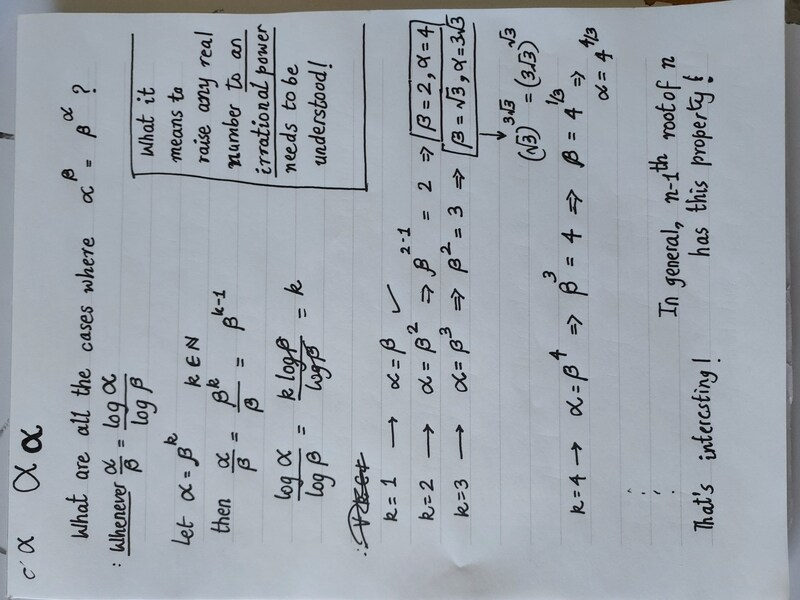
\includegraphics[width=.345\textwidth,angle=-90]{loving-to-write-by-hand-small}
\end{center}
\end{figure}

Freehand writing on a good paper with a good pen is fun. It's quick. It's rewarding.

Typesetting is, on the other hand, time-consuming and feels like \textit{Yak-shaving} \cite{Yak-shaving}. However, all good life is controlled Yak-shaving. When I typeset {\LaTeX} documents, I tend to minimize Yak-shaving and focus on having a conversation with myself. I suspect that I understand the subject matter better that way. I like the following quote in this regard:

\begin{sidebar}
I don't know what I think unless I read what I write. --Unknown
\end{sidebar}

Of course, you cannot begin solving problems on a computer. A pencil and papers are a must. In this respect, typesetting is favoring form over content. We strive to present beautifully what we have thought well but scribbled hastily. Fortunately, I don't mind taking the time to do that; it at least keeps me busy fine-tuning my thoughts. It sometimes even helps to find flaws.

However, the biggest advantage of typesetting my writing is keeping a record of beautifully typeset account of something, anything. If I could ever make a case to study under a stalwart like Professor Yaser Abu-Mostafa (\url{https://work.caltech.edu/}), or Professor Avrim Blum (\url{https://home.ttic.edu/~avrim/}), perhaps I can demonstrate what I have done in my scarce free time.

I have gone back and forth between handwritten pages and typeset manuscripts. However, I am resorting to typesetting for this work despite the overhead incurred. I hope I follow through. It's one thing to be motivated but another to be determined and disciplined.

Perhaps a picture (Figure [\ref{fig:mindmap}]) can explain better than words how I started reading Halmos's book. 

\begin{figure}[!h]
\begin{center}
\caption{A June 2025 Mindmap}
\label{fig:mindmap}
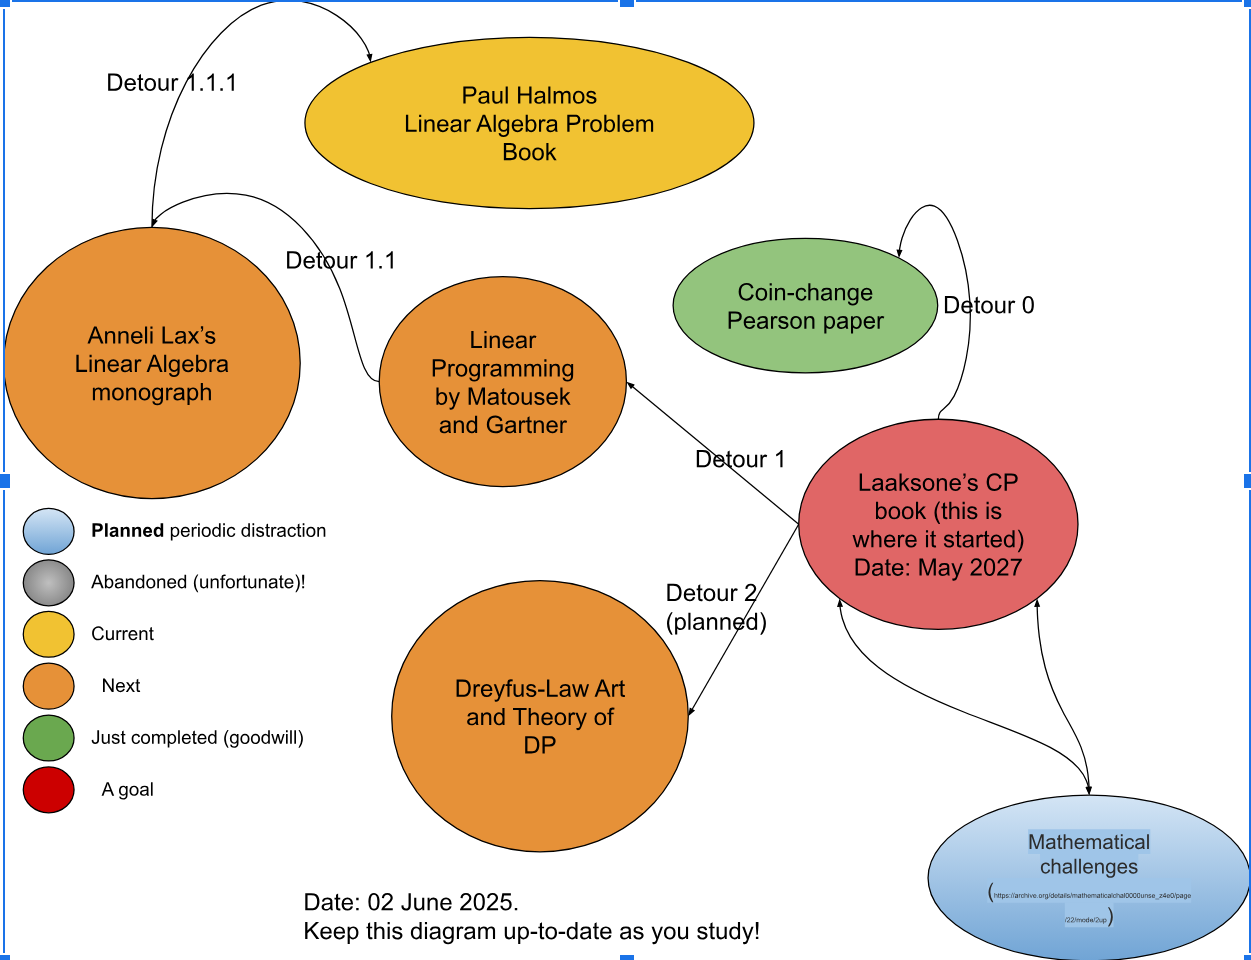
\includegraphics[width=.5\textwidth]{june-2025-mindmap}
\end{center}
\end{figure}

I will avoid answering ``Why Halmos's Linear Algebra book?'' It suffices to say that his style resonates with me, a teaser of which can be enjoyed from what follows:

\begin{sidebar}
Is it obvious that
$$ 63+48=27+84$$?
It is a true and thoroughly uninteresting mathematical statement that can be verified in a few seconds--but is it \textit{obvious}? If calling it obvious means that the reason for its truth is clearly understood, without even a single second's verification, then most people would probably say no.

What about
$$ (27+36)+48=27+(36+84)$$
?
--is that obvious?
Yes it is, for most people; the instinctive (and correct) reaction is that the way the terms of a sum are bunched together cannot affect the answer. The approved technical term is not ``bunch together'' but ``associate''; the instinctive reaction is a readiness to accept what is called the \textbf{associative law} of addition for real numbers. (Surely every reader has noticed by now that the non-obvious statement and the obvious one are in some sense the same:

$$ 63=27+36\quad and\quad 84=36+48$$)

\textbf{Linear algebra is concerned with several different kinds of operations (such as addition) on several different kinds of objects (not necessarily real numbers)}. To prepare the ground for the study of strange operations and to keep the associative law from being unjustly dismissed as a triviality, a little effort to consider some good examples and some bad ones is worthwhile.

Some of the examples will be useful in the sequel, and some won't--some are here to show that associativity can fail, and others are here to show that even when it holds it may be far from obvious. In the world of linear algebra non-associative operations are rare, but associative operations whose good behavior is not obvious are more frequently met.

\end{sidebar}

Paul Halmos has been one of my favorite authors. His insistence on problem-solving is admirable. I hope I can painstakingly (and gleefully at the same time) solve a number of problems from this book, and understand at least some of linear algebra. The problems have been solved by Halmos himself and the answers appear at the back of this book (Thank You!), but these solutions are mine. I have also felt free to think aloud, write willfully about questions that came to my mind as I solved the stated problems. That part of writing appears like `personal reflections':
\begin{reflection}
Problems come in various levels of difficulty. And, unless you are George Dantzig (who solved an open problem written on a blackboard assuming his instructor had given a homework assignment) or the like, you have to toil through them. Some you are able to solve quickly, perhaps because you are experiencing ``flow''\footnote{A highly focused mental state, defined and popularized by the psychologist Mihaly Csikszentmihalyi, conducive to productivity}, but many are challenging and you suffer (albeit purposefully) through them. They are distinct from exercises, which are also essential for fluency and emotional well-being, but expected to be easier to answer.
\end{reflection}
Feel free to skip them. As Halmos urges us in his preface to this book, I have read his solutions too. He considers solutions an integral part of exposition. The $\blacksquare$ (the QED symbol) appears after every solution. 

Readable and flawless mathematical typesetting is hard. It's ironic that the epitome of exact sciences breeds a degree of inexactness in notation. Like in literature, meaning sometimes depends on context not captured in notation. And yet, an encyclopedic treatment of notation at the beginning of a work like this tends to bore readers\footnote{What disappointments them even more are typos and errors.}. Here too, a balance needs to be sought. A few conventions are therefore in order:

\begin{itemize}
\item A roman letter in italics, like, for example, $p$, denotes an integer, unless specified otherwise.
\item The so-called \verb|\cdot|: $\cdot$ to denote multiplication is sometimes omitted. Thus, $ab$ is equivalent (and often even preferred and ubiquitous, thanks to Euler!) to $a\cdot b$.

\end{itemize}
\end{abstract}

%%%-----------------------------------------------------------------------------
\tableofcontents
%%%-----------------------------------------------------------------------------

%%%-----------------------------------------------------------------------------
\chapter{Scalars}
%%%-----------------------------------------------------------------------------
\begin{problem}
\label{pr:2a2b}
If a new addition for real numbers, denoted by the temporary symbol $\boxplus$, is defined by
$$
\alpha\boxplus\beta=2\alpha+2\beta
$$
, is $\boxplus$ associative?

Note: The $+$ sign on the right denotes ordinary addition.

Note: The new operation $\boxplus$ is \textit{commutative}: $\alpha\boxplus\beta=2\alpha+2\beta$ indeed equals $\beta\boxplus\alpha=2\beta+2\alpha$.
\end{problem}

\textbf{Solution}.

No. We can easily demonstrate 

$$
\alpha\boxplus(\beta\boxplus\gamma)\ne(\alpha\boxplus\beta)\boxplus\gamma
$$


$\blacksquare$

\begin{problem}
\label{pr:a2b}
If a new addition for real numbers, denoted by the temporary symbol $\boxplus$, is defined by
$$
\alpha\boxplus\beta=2\alpha+\beta
$$
, is $\boxplus$ associative?
\end{problem}

\textbf{Solution}.

No. We can easily demonstrate 

$$
\alpha\boxplus(\beta\boxplus\gamma)\ne(\alpha\boxplus\beta)\boxplus\gamma
$$

\begin{problem}
\label{pr:atob}
If an operation for \emph{positive integers}, denoted by the temporary symbol $*$, is defined by
$$
\alpha*\beta=\alpha^\beta
$$
, is it commutative? Is it associative?
\end{problem}

\textbf{Solution}.

Although $\alpha^\beta=\beta^\alpha$ when $\alpha=\beta$, in general, $\alpha^{\beta}$ doesn't seem to equal $\beta^\alpha$. A simple counterexample is $\alpha=1,\beta=2$. Therefore, $*$ is not a commutative operation on two positive integers.
\begin{reflection}

I asked myself, ``For which real numbers $\alpha,\beta$ (although in Problem [\ref{pr:atob}] they are positive integers) are $\alpha^\beta$ and $\beta^\alpha$ equal?''

The following exploration amazed me.
$$
\alpha^\beta=\beta^\alpha
$$
\begin{equation}
\label{eq:takelogs}
\therefore \beta\log\alpha=\alpha\log\beta
\end{equation}

\begin{equation}
\label{eq:ablogalob}
\therefore \frac{\alpha}{\beta}=\frac{\log\alpha}{\log\beta}
\end{equation}

A general solution of equation [\ref{eq:ablogalob}] (a Diophantine equation for we seek integer solutions) is perhaps hard, but somehow I asked, ``What if $\alpha=\beta^k$ for some $k\in\mathbb N$?'' I don't know why I thought of that. Is that intuition? Maybe.

Equation [\ref{eq:ablogalob}] then gives
$$
\frac{\beta^k}{\beta}=\frac{k\cancel{\log\beta}}{\cancel{\log\beta}}
$$
which simplifies to

\begin{equation}
\label{eq:bk-1k}
\beta^{k-1}=k
\end{equation}


%\begin{table}[h!]
%\centering
\begin{tabular}{|c|c|c|}
 \hline
 $k$ & What follows from $\alpha=\beta^k$ & $\alpha,\beta$ \\ \hline
 \hline
 $1$ & $\alpha=\beta$  & Any real numbers \\ \hline
 $2$ & $\beta^{2-1}=\beta=2$ & $\alpha=4,\beta=2$ \\ \hline
 $3$ & $\beta^{3-1}=\beta^2=3$ & $\alpha=3\sqrt{3},\beta=\sqrt{3}$ \\ \hline
 $4$ & $\beta^{4-1}=\beta^3=4$ & $\alpha=4\sqrt[3]{4},\beta=\sqrt[3]{4}$ \\ \hline
\end{tabular}

%\caption{When does $\alpha^\beta=\beta^\alpha$ if $\alpha=\beta^k, k\in\mathbb N$?}
%\label{tab:ab=ba}
%\end{table}

That was interesting! 

\end{reflection}

Exponentiation is associative only when $\beta\gamma=\beta^\gamma$. There are specific cases when that is true (e.g. $\beta=\gamma=2$), but it is not true in general. A simple counterexample is $\alpha=2,\beta=1,\gamma=3$.


Problem [\ref{pr:atob}] shows that ``natural'' operations can fail to be associative.

Halmos introduces complex numbers simply as a ``pair of real numbers'':$\langle\alpha,\beta\rangle\mid\alpha,\beta\in\mathbb{R}$. We can then \textit{define} operations of interest on them, and examine if they are commutative and associative.

An operation $\boxplus$ defined on complex numbers $\langle\alpha,\beta\rangle$ and $\langle\gamma,\delta\rangle$ as:

$$
\langle\alpha,\beta\rangle\boxplus\langle\gamma,\delta\rangle=\langle\alpha+\gamma,\beta+\delta\rangle
$$
is commutative and associative because the addition of real numbers is so. The result of this operation is also a complex number.


\begin{problem}
\label{pr:complexmult}
If an operation for the ordered pair of real numbers, denoted by the temporary symbol $\boxdot$, is defined by
$$
\langle\alpha,\beta\rangle\boxdot\langle\gamma,\delta\rangle=\langle\alpha\gamma-\beta\delta,\alpha\delta+\beta\gamma\rangle
$$
, is it commutative? Is it associative?
\end{problem}
\textbf{Solution}.

The $\boxdot$ operation is indeed commutative because the addition and multiplication of real numbers are.

\begin{align*}
\langle\gamma,\delta\rangle\boxdot\langle\alpha,\beta\rangle
&=
\langle\gamma\alpha-\delta\beta,\gamma\beta+\delta\alpha\rangle \\
&=\langle\alpha\gamma-\beta\delta,\alpha\delta+\beta\gamma\rangle\\
&=\langle\alpha,\beta\rangle\boxdot\langle\gamma,\delta\rangle
\end{align*}
Still, we are lucky! It wouldn't be commutative had it been defined just a little differently as:
$\langle\alpha,\beta\rangle\boxdot\langle\gamma,\delta\rangle=\langle\alpha\gamma+\beta\delta,\alpha\delta-\beta\gamma\rangle$

Associativity:
\begin{align*}
(\langle a, b\rangle\boxdot\langle c, d\rangle)\boxdot\langle m, n\rangle
&=
\langle a c- b d, a d+ b c\rangle\boxdot\langle m, n\rangle\\
&=\langle(ac-bd)m-(ad+bc)n,(ac-bd)n+(ad+bc)n\rangle
\end{align*}


%%%-----------------------------------------------------------------------------
%%%-----------------------------------------------------------------------------
\MakeBibliography[nosplit]
%%%-----------------------------------------------------------------------------

%%%-----------------------------------------------------------------------------
\end{document}
%%%-----------------------------------------------------------------------------
